\section{Locality, Weight Sharing, and the Logic of Convolution}

Section 3.1 argued that architecture matters because it encodes structural assumptions directly into the hypothesis class.
Convolution is one of the clearest and most influential examples of that principle.
It does not merely provide a convenient implementation for image processing.
It expresses, in mathematically explicit form, three linked assumptions:
local interactions matter,
similar local patterns may recur across position,
and larger-scale structure may be built hierarchically from smaller-scale features.

\medskip

This section develops those ideas in a more formal way.
We will define discrete convolution in one and two dimensions, show that it is a linear operator with highly structured matrix form, prove its translation-equivariance property, compare its parameter count with that of dense layers, and derive how receptive fields grow across stacked layers.
The broader lesson is that convolution achieves statistical efficiency by restricting the model to a structured subclass of linear maps before nonlinearity is even applied.

\subsection*{Discrete convolution in one and two dimensions}

We begin with formal definitions.

\begin{definition}[One-dimensional discrete convolution]
Let $x \in \mathbb{R}^n$ be a one-dimensional signal and let $w \in \mathbb{R}^k$ be a kernel of width $k$.
For indices at which the expression is defined, the discrete convolution of $x$ by $w$ is the signal $y = w * x$ given by
\[
 y_i = (w*x)_i = \sum_{t=0}^{k-1} w_t\, x_{i-t}.
\]
Depending on the boundary convention, one may use zero padding, valid convolution, circular indexing, or other extensions.
\end{definition}

\begin{definition}[Two-dimensional discrete convolution]
Let $X \in \mathbb{R}^{H \times W}$ be an image and let $K \in \mathbb{R}^{r \times s}$ be a two-dimensional kernel.
For indices at which the expression is defined, the discrete convolution of $X$ by $K$ is the array $Y = K * X$ with entries
\[
 Y_{i,j} = (K*X)_{i,j} = \sum_{u=0}^{r-1}\sum_{v=0}^{s-1} K_{u,v}\, X_{i-u,j-v}.
\]
Again, the precise output shape depends on the boundary convention and any padding rule.
\end{definition}

\medskip

In practice, deep-learning libraries sometimes implement cross-correlation rather than strict mathematical convolution, since the kernel may be applied without reversal.
For the structural questions that matter here --- locality, parameter sharing, and equivariance --- that distinction is not essential.
The key point is that each output coordinate depends only on a local neighborhood of the input, and that the same coefficients are reused at every position.

\subsection*{Convolution as a structured linear operator}

Convolution is often introduced as a sliding-window procedure.
But for mathematical analysis it is better understood as a special kind of linear map.

\begin{proposition}[Convolution is a linear operator with Toeplitz structure]
For fixed kernel $w \in \mathbb{R}^k$, the map
\[
 x \longmapsto w * x
\]
from signals to signals is linear.
Under standard zero-padding or valid-convolution conventions, its matrix representation in one dimension is Toeplitz up to boundary effects.
Under circular boundary conditions it is circulant.
In two dimensions, the corresponding matrix form is block Toeplitz with Toeplitz blocks.
\end{proposition}

\begin{proof}
Linearity is immediate from the definition.
For scalars $a,b$ and signals $x,z$,
\[
 w*(ax+bz)
 = \sum_t w_t(ax_{i-t}+bz_{i-t})
 = a\sum_t w_t x_{i-t} + b\sum_t w_t z_{i-t}
 = a(w*x)+b(w*z).
\]

To obtain the matrix form in one dimension, write the convolution as multiplication by a matrix $T_w$ whose $i$th row contains the kernel coefficients aligned with the input coordinates contributing to output position $i$.
Because shifting the output index shifts the alignment pattern by one step, the entries along each diagonal are equal.
That is exactly the Toeplitz property.
Under circular indexing the diagonals wrap around, producing a circulant matrix.

In two dimensions, vectorizing the image turns convolution into multiplication by a matrix whose blocks correspond to horizontal shifts and whose entries inside each block correspond to vertical shifts.
The repeated shift pattern yields a block-Toeplitz matrix with Toeplitz blocks.
\end{proof}

\medskip

This proposition is conceptually important.
A dense layer is also linear before the activation function, but it allows every output coordinate to depend on every input coordinate with an independent coefficient.
Convolution is more restrictive.
It selects a very special subclass of linear maps: those that are sparse because of locality and repetitive because of weight sharing.
That restriction is not a defect.
It is the source of the model's inductive bias and one of the main reasons it can learn effectively from realistic sample sizes.

\subsection*{Locality and weight sharing as structural bias}

Two ideas work together in convolution.

\paragraph{Locality.}
Each output unit sees only a small neighborhood of the input.
In a one-dimensional kernel of width $k$, output coordinate $y_i$ depends on at most $k$ nearby coordinates of $x$.
In a two-dimensional $r \times s$ kernel, output location $(i,j)$ depends only on an $r \times s$ patch.
This forbids arbitrary long-range interaction at a single layer.

\paragraph{Weight sharing.}
The same kernel coefficients are reused across positions.
A local edge detector, texture detector, or short phrase detector does not need separate parameters for every possible location.
Once the architecture assumes that the same pattern may occur anywhere, it becomes natural to tie those parameters together.

\medskip

These two constraints jointly explain why convolution is statistically efficient.
The model does not waste parameters on learning a separate detector for every coordinate, and it does not try to model every possible pairwise interaction at once.
Instead, it begins with a simpler structural prior and then compounds that prior across depth.

\begin{figure}[t]
\centering
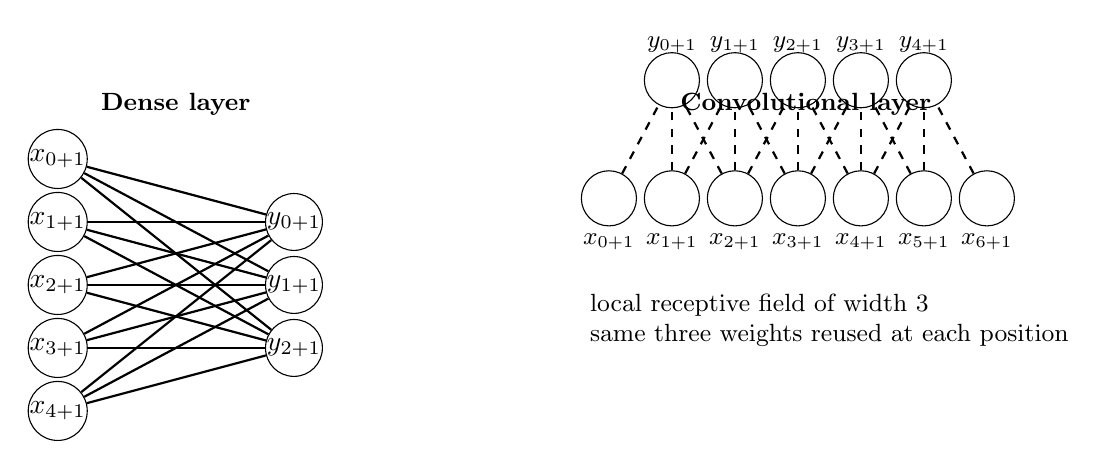
\begin{tikzpicture}[x=1cm,y=1cm,
    inode/.style={draw, circle, minimum size=7mm, inner sep=0pt},
    onode/.style={draw, circle, minimum size=7mm, inner sep=0pt},
    conn/.style={thick},
    shared/.style={thick, dashed},
    lbl/.style={font=\small}
]

% left: dense connectivity
\node[lbl] at (1.5,2.7) {\textbf{Dense layer}};
\foreach \i in {0,...,4} {
  \node[inode] (d\i) at (0,2-\i*0.8) {$x_{\i+1}$};
}
\foreach \j in {0,...,2} {
  \node[onode] (u\j) at (3,1.2-\j*0.8) {$y_{\j+1}$};
}
\foreach \i in {0,...,4} {
  \foreach \j in {0,...,2} {
    \draw[conn] (d\i) -- (u\j);
  }
}

% right: local + shared
\node[lbl] at (9.5,2.7) {\textbf{Convolutional layer}};
\foreach \i in {0,...,6} {
  \node[inode] (c\i) at (7+\i*0.8,1.5) {};
  \node[lbl] at (7+\i*0.8,0.95) {$x_{\i+1}$};
}
\foreach \j in {0,...,4} {
  \node[onode] (z\j) at (7.8+\j*0.8,3.0) {};
  \node[lbl] at (7.8+\j*0.8,3.45) {$y_{\j+1}$};
}
\foreach \j in {0,...,4} {
  \pgfmathtruncatemacro{\a}{\j}
  \pgfmathtruncatemacro{\b}{\j+1}
  \pgfmathtruncatemacro{\cidx}{\j+2}
  \draw[shared] (c\a) -- (z\j);
  \draw[shared] (c\b) -- (z\j);
  \draw[shared] (c\cidx) -- (z\j);
}
\node[lbl, align=left] at (9.8,-0.05) {local receptive field of width $3$\\same three weights reused at each position};
\end{tikzpicture}
\caption{Locality and weight sharing contrasted with dense connectivity.
A dense layer permits every output to depend on every input with independent coefficients.
A convolutional layer restricts each output to a local neighborhood and reuses the same kernel across positions.}
\label{fig:conv-locality-sharing}
\end{figure}

\subsection*{Translation equivariance}

One of the most mathematically attractive properties of convolution is translation equivariance.
Intuitively, if the input pattern shifts, the feature map shifts in the same way.
The detector therefore responds consistently across location.

To state this carefully, define the translation operator $T_a$ on one-dimensional signals by
\[
 (T_a x)_i = x_{i-a}.
\]
A similar definition applies in two dimensions by shifting both coordinates.

\begin{theorem}[Translation equivariance of discrete convolution]
Let $w$ be a fixed one-dimensional convolution kernel, and let $T_a$ denote translation by offset $a$ on signals indexed so that the operations are well-defined under a common boundary convention.
Then
\[
 w * (T_a x) = T_a (w*x)
\]
for every signal $x$.
Thus discrete convolution is translation equivariant.
The same statement holds in two dimensions with respect to spatial translations.
\end{theorem}

\begin{proof}
Compute the $i$th output coordinate:
\[
 (w*(T_a x))_i = \sum_t w_t (T_a x)_{i-t} = \sum_t w_t x_{i-t-a}.
\]
On the other hand,
\[
 (T_a(w*x))_i = (w*x)_{i-a} = \sum_t w_t x_{(i-a)-t} = \sum_t w_t x_{i-t-a}.
\]
The two expressions are identical for every $i$, so
\[
 w*(T_a x) = T_a(w*x).
\]
The two-dimensional proof is the same, with the translation acting on both spatial indices.
\end{proof}

\medskip

This theorem helps explain why convolution is so natural for images and other spatial data.
If a feature such as an edge, corner, or local texture moves in the image, the representation produced by the convolutional layer moves with it rather than changing unpredictably.
The model therefore does not need to relearn essentially the same detector at each possible location.

It is worth stressing the distinction between equivariance and invariance.
A convolutional feature map is typically equivariant: shifting the input shifts the feature map.
A classification system may become approximately invariant only after subsequent aggregation steps such as pooling, striding, or global averaging reduce sensitivity to exact position.

\subsection*{Parameter efficiency: dense versus convolutional layers}

The statistical advantage of convolution becomes especially visible when one counts parameters.
Suppose first that an image $X \in \mathbb{R}^{H \times W \times C_{\mathrm{in}}}$ is flattened into a vector and passed into a dense layer with $M$ output units.
Then the weight matrix has
\[
M \cdot HWC_{\mathrm{in}}
\]
free parameters, plus $M$ bias terms.
Every output unit has its own full set of coefficients.

Now consider a convolutional layer with kernel size $r \times s$, $C_{\mathrm{in}}$ input channels, and $C_{\mathrm{out}}$ output channels.
Its parameter count is
\[
 r s\, C_{\mathrm{in}} C_{\mathrm{out}}
\]
for the kernel coefficients, plus $C_{\mathrm{out}}$ bias terms.
Crucially, this count is independent of the spatial dimensions $H$ and $W$.
The same filter bank is reused across all locations.

\medskip

For large images the contrast can be dramatic.
If $H=W=128$, $C_{\mathrm{in}}=3$, and one wants $C_{\mathrm{out}}=64$ output channels with a $3\times 3$ kernel, then a convolutional layer uses
\[
3\cdot 3\cdot 3\cdot 64 = 1728
\]
weights, while even a modest dense layer producing one scalar at every spatial location would require a number of parameters proportional to $128^2$ times the number of outputs.
The exact comparison depends on the output shape, but the principle is universal:
convolution decouples parameter count from spatial extent because it assumes translation reuse.

\begin{proposition}[Locality and weight sharing reduce degrees of freedom]
Consider a single linear layer acting on an input image with spatial size $H \times W$ and $C_{\mathrm{in}}$ channels, producing $C_{\mathrm{out}}$ output channels.
A dense layer that treats each output location independently requires a number of free linear parameters that scales with $HW$.
A convolutional layer with fixed kernel size $r \times s$ requires only $rs\, C_{\mathrm{in}} C_{\mathrm{out}}$ parameters, independent of $H$ and $W$.
Therefore locality and weight sharing reduce the number of free degrees of freedom whenever the spatial domain contains more than one receptive field position.
\end{proposition}

\begin{proof}[Proof sketch]
The dense layer assigns an independent coefficient to each admissible input--output pair, so the number of parameters scales with the number of output positions times the number of input coordinates influencing each output.
A convolutional layer instead uses the same $r \times s$ local coefficient tensor at every output position.
Thus once the kernel size and channel counts are fixed, spatial replication creates additional applications of the same parameters rather than new parameters.
For any nontrivial spatial domain, that yields fewer independent degrees of freedom than the corresponding untied dense map.
\end{proof}

\medskip

This is a particularly clear instance of the general principle from Section 3.1:
architecture restricts the admissible function class.
Convolution does not search among all linear maps from images to feature maps.
It searches among those compatible with locality and translation reuse.
That restriction lowers parameter count, reduces variance, and often improves sample efficiency when the assumptions are well matched to the data.

\subsection*{Receptive fields and hierarchical growth}

A single convolutional layer is local.
But deep convolutional networks are not merely local detectors.
Their effective scope grows with depth.
This is captured by the idea of the receptive field.

\begin{definition}[Receptive field]
The \emph{receptive field} of a unit in a layered architecture is the subset of input coordinates that can influence that unit.
For a convolutional layer, the immediate receptive field is determined by the kernel support.
For a stack of layers, the receptive field is obtained by composing these local dependencies across depth.
\end{definition}

For stride-$1$ convolutions with kernel widths $k_1,\dots,k_L$ and no dilation, the receptive field size after $L$ layers in one dimension is
\[
R_L = 1 + \sum_{\ell=1}^{L} (k_{\ell}-1).
\]
In particular, if all layers use the same kernel width $k$, then
\[
R_L = 1 + L(k-1).
\]
Thus repeated local operations gradually create larger effective context.

More generally, with strides $s_1,\dots,s_L$, one obtains the recursion
\[
R_1 = k_1,
\qquad
R_{\ell} = R_{\ell-1} + (k_{\ell}-1)\prod_{j=1}^{\ell-1} s_j,
\qquad \ell \ge 2.
\]
This expression shows how downsampling causes later layers to aggregate information over increasingly large regions of the original input.

\begin{figure}[t]
\centering
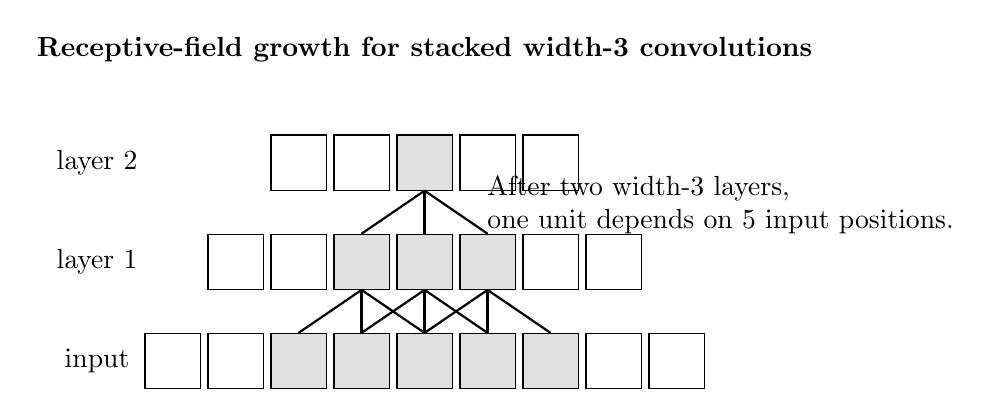
\begin{tikzpicture}[x=0.8cm,y=0.9cm,
    cell/.style={draw, minimum width=0.7cm, minimum height=0.7cm, inner sep=0pt},
    hi/.style={draw, minimum width=0.7cm, minimum height=0.7cm, inner sep=0pt, fill=black!12}
]

\node at (4,4.4) {\textbf{Receptive-field growth for stacked width-3 convolutions}};

% input row
\foreach \i in {0,...,8} {
  \node[cell] (x\i) at (\i,0) {};
}
\node at (-1.2,0) {input};

% layer1
\foreach \i in {0,...,6} {
  \node[cell] (h\i) at (\i+1,1.4) {};
}
\node at (-1.2,1.4) {layer 1};

% layer2
\foreach \i in {0,...,4} {
  \node[cell] (g\i) at (\i+2,2.8) {};
}
\node at (-1.2,2.8) {layer 2};

% highlight one output and dependencies
\node[hi] (g2) at (4,2.8) {};
\node[hi] (h1) at (3,1.4) {};
\node[hi] (h2) at (4,1.4) {};
\node[hi] (h3) at (5,1.4) {};
\foreach \i in {2,...,6} {
  \node[hi] (xx\i) at (\i,0) {};
}

\draw[thick] (g2.south) -- (h1.north);
\draw[thick] (g2.south) -- (h2.north);
\draw[thick] (g2.south) -- (h3.north);
\foreach \i/\j in {1/2,1/3,1/4,2/3,2/4,2/5,3/4,3/5,3/6} {
  \draw[thick] (h\i.south) -- (x\j.north);
}

\node[align=left] at (8.7,2.2) {After two width-$3$ layers,\\one unit depends on $5$ input positions.};
\end{tikzpicture}
\caption{Stacking local convolutions enlarges the receptive field.
Although each individual layer is local, depth allows later units to integrate information over larger regions of the original input.}
\label{fig:conv-receptive-field}
\end{figure}

\medskip

This is the heart of the hierarchical story.
Early layers may detect edges, corners, short motifs, or small textures.
Later layers combine those local responses into larger parts, configurations, and semantic structures.
Convolutional networks therefore achieve nonlocal expressivity not by abandoning locality, but by composing it repeatedly.

\subsection*{A worked one-dimensional example}

A small example makes the structure concrete.

\begin{example}[Convolution on a tiny one-dimensional signal]
Consider the signal
\[
 x = (2,1,0,3,1)
\]
and the kernel
\[
 w = (1,-1).
\]
Using valid convolution, the output has length $4$ and is given by
\[
 (w*x)_i = x_i - x_{i+1}.
\]
Hence
\[
 w*x = (2-1,\,1-0,\,0-3,\,3-1) = (1,1,-3,2).
\]
This kernel acts as a simple local difference detector.
It responds strongly where adjacent entries change sharply.

Now shift the input by one position to obtain
\[
 T_1x = (0,2,1,0,3,1)
\]
under a suitable padding convention.
Convolving again with the same kernel produces the same pattern of local differences, shifted accordingly.
This is exactly the translation-equivariance property proved above.
\end{example}

\medskip

Even this trivial example illustrates the key ideas.
The output at each position depends only on a local pair of inputs.
The same detector is applied everywhere.
And the detector moves consistently with shifts in the signal.
A dense layer could represent the same mapping, but it would not encode any of these structural facts directly.

\subsection*{Pooling and the move toward coarse invariance}

Convolutional architectures often interleave convolution with pooling or downsampling.
Pooling does not preserve full equivariance in the exact same form, but it helps aggregate nearby responses into coarser summaries.
This can make the representation less sensitive to small input translations and enlarge the effective receptive field of later layers.

\begin{figure}[t]
\centering
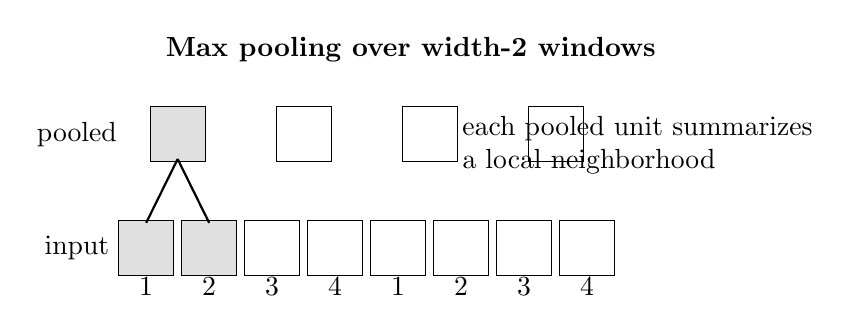
\begin{tikzpicture}[x=0.8cm,y=0.9cm,
    cell/.style={draw, minimum width=0.7cm, minimum height=0.7cm, inner sep=0pt},
    hi/.style={draw, minimum width=0.7cm, minimum height=0.7cm, inner sep=0pt, fill=black!12}
]
\node at (4.2,2.8) {\textbf{Max pooling over width-2 windows}};
\foreach \i in {0,...,7} {
  \node[cell] (a\i) at (\i,0) {};
  \node at (\i,-0.55) {$\pgfmathparse{int(mod(\i,4)+1)}\pgfmathresult$};
}
\node at (-1.1,0) {input};
\foreach \i in {0,...,3} {
  \node[cell] (b\i) at (0.5+2*\i,1.6) {};
}
\node at (-1.1,1.6) {pooled};
\node[hi] at (0,0) {};
\node[hi] at (1,0) {};
\node[hi] at (0.5,1.6) {};
\draw[thick] (0,0.35) -- (0.5,1.25);
\draw[thick] (1,0.35) -- (0.5,1.25);
\node[align=left] at (7.8,1.45) {each pooled unit summarizes\\a local neighborhood};
\end{tikzpicture}
\caption{Pooling aggregates nearby activations into a coarser representation.
This reduces spatial resolution, increases the effective scale of later features, and can create partial robustness to small translations.}
\label{fig:conv-pooling}
\end{figure}

\medskip

Pooling should be interpreted carefully.
It is not magic invariance.
Rather, it is one mechanism by which exact local location is deemphasized in favor of more stable coarse structure.
Modern architectures sometimes replace explicit pooling by strided convolutions or attention-like aggregation, but the underlying goal remains familiar: build increasingly global representations from local evidence.

\subsection*{Why structure yields statistical efficiency}

We may now state the larger lesson explicitly.
Convolution works well when the world approximately obeys the assumptions that convolution encodes.
If local patterns recur across position, then weight sharing is sensible.
If nearby coordinates interact more strongly than distant ones, then local connectivity is sensible.
If larger structures are built from smaller ones, then stacked local layers are sensible.

\medskip

When those assumptions are approximately correct, the reduction in degrees of freedom is not merely computationally convenient.
It improves learning.
The architecture no longer wastes sample complexity on rediscovering the same local detector at every location.
It no longer spends parameters expressing arbitrary global couplings at the first layer.
Instead, it searches within a function class aligned with the geometry of the task.
That is exactly what one hopes from inductive bias.

\medskip

This point also clarifies the limits of convolution.
If the task depends primarily on nonlocal interactions, arbitrary permutations, or long-range relations that are not naturally built from local patterns, then convolution alone may be too restrictive.
The power of convolution comes from matching the structure of the domain.
Its success is therefore not universal; it is conditional on the usefulness of locality and translation reuse.

\subsection*{Notes and references}

The mathematical view of convolution as a structured linear operator connects deep learning to classical signal processing and harmonic analysis.
Standard signal-processing texts develop discrete convolution, Toeplitz structure, and the convolution theorem in more classical language.
In the deep-learning literature, the central role of convolutional architectures in vision was established by LeCun and collaborators and later synthesized in modern textbooks such as Goodfellow, Bengio, and Courville.

\medskip

The importance of translation equivariance and local receptive fields is now understood as part of a broader symmetry-based view of architecture.
That perspective connects naturally to later developments in group-equivariant neural networks and geometric deep learning.
For the purposes of this chapter, however, the main message is already visible in the elementary formulas of this section:
convolution is a deliberately restricted hypothesis class, and that restriction is precisely what makes it powerful on the right domains.
